\chapter{Introducción}
\label{cap:capitulo1}
\setcounter{page}{1}

Desde sus inicios, la robótica ha proporcionado un sinfín de posibilidades y alternativas ante problemas que anteriormente carecían de las soluciones adecuadas, pero, ¿qué es realmente la robótica?\\

Se podría definir robótica como el proceso mediante el cual una máquina intercambia energía e información con su entorno, con el propósito de alcanzar una serie de objetivos específicos. Este campo tecnológico en expansión es el resultado de décadas de colaboración continua entre biólogos, informáticos e ingenieros \cite{Koditschek21}. Dada esta multidisciplina, la robótica abarca una amplia gama de aplicaciones, desde la industria hasta la medicina, pasando por la exploración espacial, la domótica o la conducción autónoma, entre otras. Es un campo en constante evolución, impulsado por la búsqueda de soluciones innovadoras para mejorar la calidad de vida y permitir superar desafíos de manera más eficiente y segura.\\

La industria agrícola no es una excepción, ya que ha contemplado históricamente tareas que requieren una dedicación laboral considerable. No obstante, gracias a la robótica y a los sistemas de visión artificial, surge la oportunidad de transformar una serie de procesos, como puede ser la recolección de cultivos a través de la detección automatizada.\\

En las siguientes secciones describiremos brevemente algunas de las aplicaciones más importantes de la robótica en la sociedad actual, así como los distintos conceptos en los cuales se basa la investigación y el desarrollo llevado a cabo.\\

\section{Robots y robótica}
\label{sec:robótica} % etiqueta para luego referenciar esta sección

Según la Federación Internacional de Robots (IFR) se define robot según el vocabulario establecido por la International Organization for Standardization (ISO), y esto es como \textit{mecanismo accionado programado con cierto grado de autonomía para realizar tareas de locomoción, manipulación o posicionamiento} \cite{ISO8373}.\\  

El término robot fue utilizado por primera vez por Karel Capek (en su obra de teatro Rossum’s Universal Robots publicada en 1920. Esta palabra viene del vocablo checo \textit{“robota”} que significa trabajo, en el sentido de la obligatoriedad, entendido como servidumbre, trabajo forzado o esclavitud \cite{Sanchez07a}. Aunque esta definición es un punto de partida, es cierto que es posible diferir en aspectos como si un robot debe controlarse automáticamente o podría ser autónomo o si un robot debe ser reprogramable. A un nivel más amplio, cualquier máquina que pueda utilizarse para llevar a cabo acciones o tareas complejas de forma automática puede considerarse un robot \cite{Raj19}.\\

Históricamente, las civilizaciones antiguas, como la egipcia y la griega, dieron los primeros pasos en lo que se puede denominar robótica clásica, construyendo autómatas y mecanismos diseñados para imitar acciones humanas, con características mecánicas rudimentarias. 
Con el paso del tiempo, la ciencia y la ingeniería avanzaron, y los conceptos de la robótica comenzaron a tomar forma más definida hasta que, en el siglo XX, con el desarrollo de la ingeniería en sus diferentes ramas (mecánica, electrónica, informática, telecomunicaciones), Isaac Asimov (1920-1992) utilizó por primera vez el término robótica y postuló las tres leyes de la robótica en su libro \textit{I Robot} publicado en 1950, coincidiendo con el apogeo de la robótica moderna. Asimov consideró necesario añadir una cuarta ley, antepuesta a las demás, la número cero, que afirma que un robot no debe actuar simplemente para satisfacer intereses individuales, sino que sus acciones deben preservar el beneficio común de toda la humanidad \cite{Sanchez07b}.\\

Es también en 1950 cuando Alan Mathison Turing publica \textit{Computing Machinery and Intelligence} y propone una prueba (test o máquina de Touring), en forma de entidad matemática abstracta, que demuestra la existencia de problemas computacionales irresolubles que ninguna máquina es capaz de solventar. Se puede afirmar que un programa de ordenador no llegará nunca a ser tan inteligente como un ser humano y que un robot no podrá suplir al ser humano de forma completa \cite{Sanchez07b} preocupación sobre el potencial de sustitución de la mano de obra, que históricamente ha atenuado el entusiasmo en torno a las nuevas tecnologías \cite{Mokyr15}.\\

Partiendo de todos estos avances y del interés por automatizar las tareas de producción, la robótica va adquiriendo un gran desarrollo \cite{Sanchez07b}. Es debido a este desarrollo que, atendiendo al propósito y al contexto en el que se utilicen estos robots, se fueron creando varios grupos en función de los que clasificarlos. Estos tres grandes grupos fueron, en función de una serie de criterios generales: robots industriales, robots de servicio y robots médicos.

\subsection{Robots industriales}
\label{sec:robots_industriales}

Se define robot industrial como un manipulador polivalente, reprogramable y controlado automáticamente, programable en tres o más ejes, que puede ser fijo o móvil para su uso en aplicaciones de automatización industrial \cite{ISO8373}.\\

El inicio de la robótica industrial puede datarse en la década de 1950, aunque algunos tipos de automatización en el entorno industrial empezaron a aparecer desde los tiempos de la Revolución Industrial. La evolución de los robots industriales puede subdividirse en cuatro categorías: las tres primeras abarcan el período comprendido entre los años cincuenta y finales de los noventa, mientras que la cuarta generación abarca desde 2000 hasta nuestros días \cite{Gasparetto19}.\\

La primera generación, o primeros manipuladores (1950-1967), eran básicamente máquinas programables que no tenían comunicación con el entorno externo y con algoritmos de control sencillos (punto a punto). En cuanto al hardware, contaban con equipos de baja tecnología, sin servo-controladores. Sin embargo, en 1954, George Devol y Joseph Engelberger formaron la empresa Unimation, empresa que desarrollaría Unimate (ver en Figura \ref{fig:primer_robot_industrial}), considerado el primer robot industrial de la historia, fabricado en 1961 \cite{Zamalloa17}.
  
  \begin{figure}[H]
    \begin{center}
      \subcapcentertrue
      \subfigure[Joseph Engelberger y George Devol]{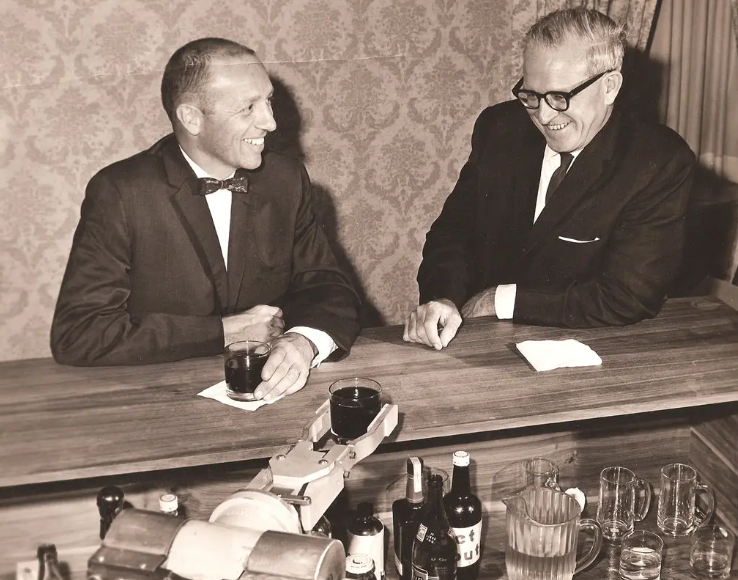
\includegraphics[width=62mm]{figs/Engelberger_Devol.png}}
      \hspace{2mm}
      \subfigure[Robot Unimate]{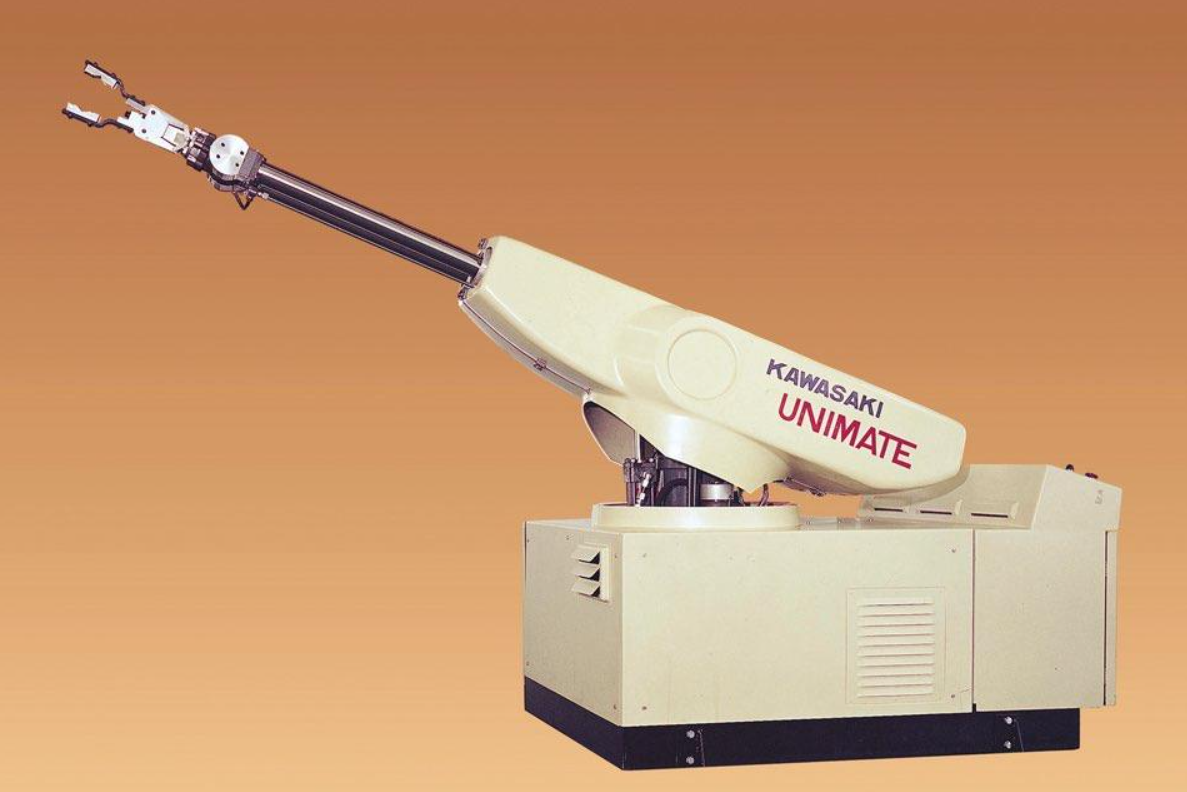
\includegraphics[width=73mm]{figs/Unimate robot.png}}
    \end{center}
    \caption{Primer robot industrial}
    \label{fig:primer_robot_industrial}
  \end{figure}
  
Empresas como Ford y General Motors empezaron a plantearse la automatización de sus plantas productivas, por lo que, en 1962, la empresa AMF Corporation fabricó un nuevo robot llamado Versatan, un robot cilíndrico que Ford encargó para sus fábricas. Este robot, fue también el primero que se instaló en un centro productivo en Japón \cite{Gasparetto19}. \\

La segunda generación, o robots sensorizados (1968-1977), eran máquinas programables básicas con posibilidades limitadas de comportamiento autoadaptativo y capacidades elementales para reconocer el entorno externo, poseían sistemas sensoriales avanzados y eran robots de gran volumen que se utilizaban principalmente en automoción \cite{Zamalloa17}. \\

En 1968, en el Stanford Artificial Intelligence Laboratory (SAIL) se confecciona el WAVE, el primer lenguaje de programación para robots. En 1969, Unimation concedió a Kawasaki Heavy Industries Ltd. la licencia para producir robots para el mercado japonés y asiático, conduciendo al desarrollo del Kawasaki-Unimate 2000, el primer robot industrial construido en Japón. Es también en este año cuando Víctor Scheinman, un estudiante de ingeniería mecánica de la Universidad de Standford, diseñó y construyó el primer prototipo de brazo robótico (Figura \ref{fig:standford_arm}), cuya cinemática inversa podía resolverse de manera analíticamente cerrada, permitiendo una rápida ejecución de la trayectoria \cite{Gasparetto19}. \\

  \begin{figure}[H]
    \begin{center}
      \subcapcentertrue
      \subfigure[Victor Scheinman con el Standford Arm]{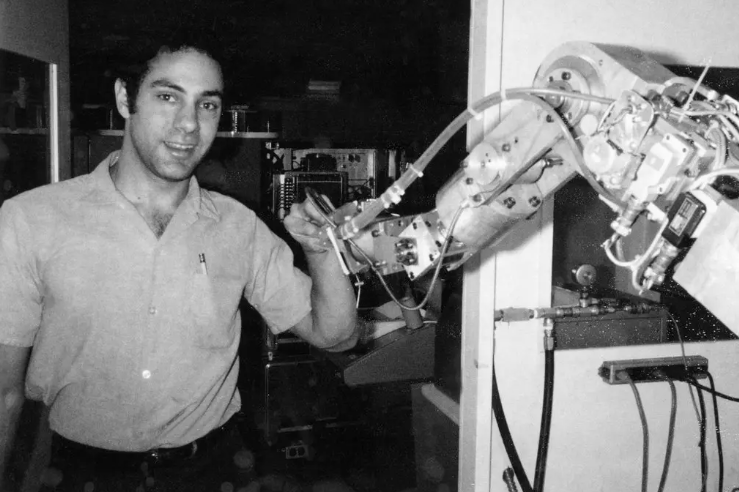
\includegraphics[width=62mm]{figs/Victor_Scheinman.png}}
      \hspace{2mm}
      \subfigure[Standford Arm]{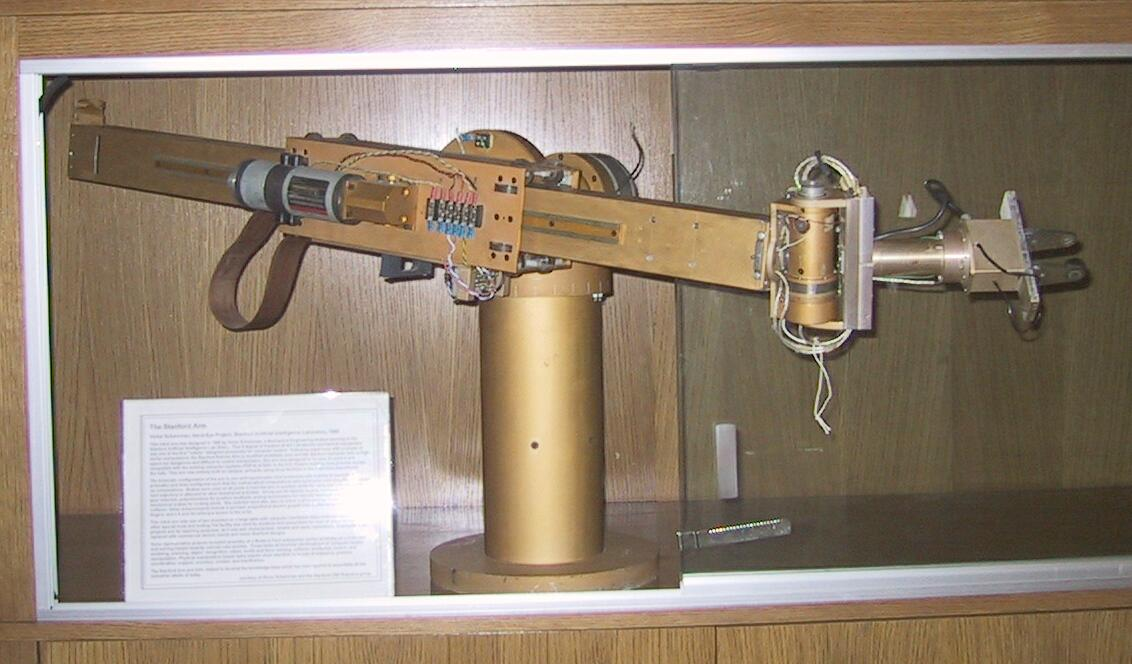
\includegraphics[width=71mm]{figs/Standford_arm.jpeg}}
    \end{center}
    \caption{Standford Arm}
    \label{fig:standford_arm}
  \end{figure}
 
En 1969, el ingeniero de la compañía Yaskawa, T Mori, acuña el término mecatrónica, que integra el conjunto de mecanismos de control automático imprescindibles para el desarrollo de cualquier máquina inteligente \cite{Sanchez07b} tal y como muestra el diagrama de la Figura \ref{fig:Mecatrónica}.
  
  \begin{figure} [h!]
    \begin{center}
      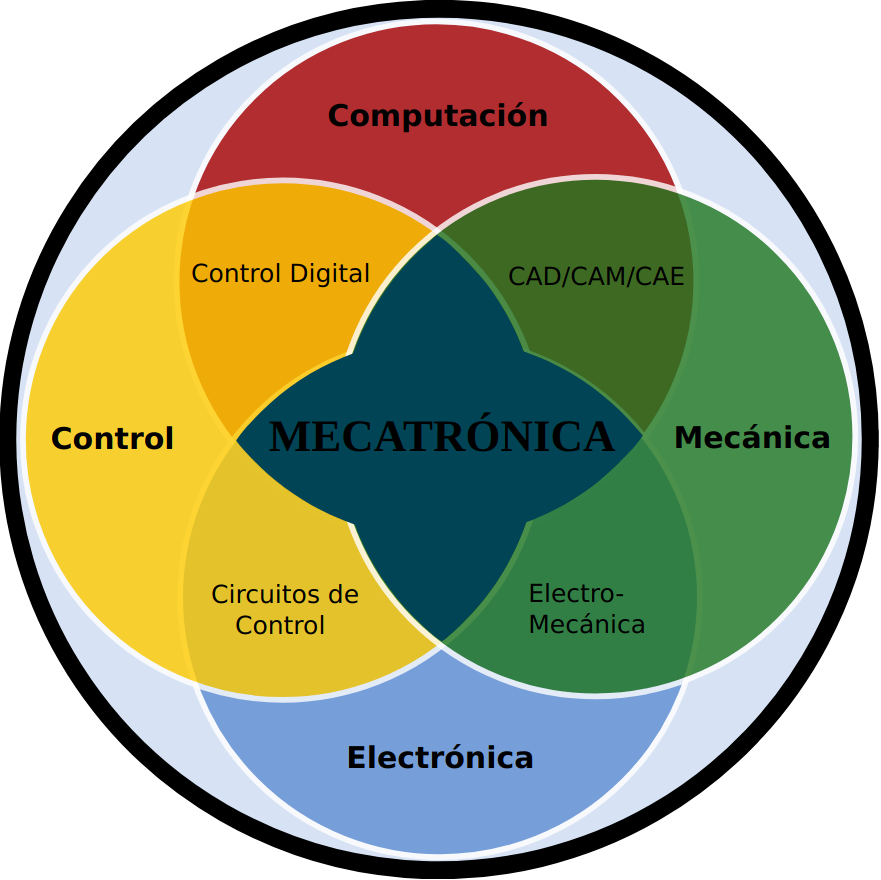
\includegraphics[width=65mm]{figs/meca.png}
    \end{center}
    \caption{Diagrama mecatrónico de construcción de máquinas inteligentes}
    \label{fig:Mecatrónica}
  \end{figure}
  
En 1973, KUKA  \footnote{\url{https://www.kuka.com/es-es}} construyó el primer robot industrial con 6 ejes electromecánicos llamado Famulus. Un año más tarde, Cincinnati Milacron introdujo en el mercado el robot T3 (Figura \ref{fig:T3}). Cincinnati Milacron (adquirida por ABB \footnote{\url{https://new.abb.com/products/robotics}} en 1990). El robot T3 fue el primer robot comercial controlado por un microordenador \cite{Zamalloa17}.\\
  
  \begin{figure} [H]
    \begin{center}
      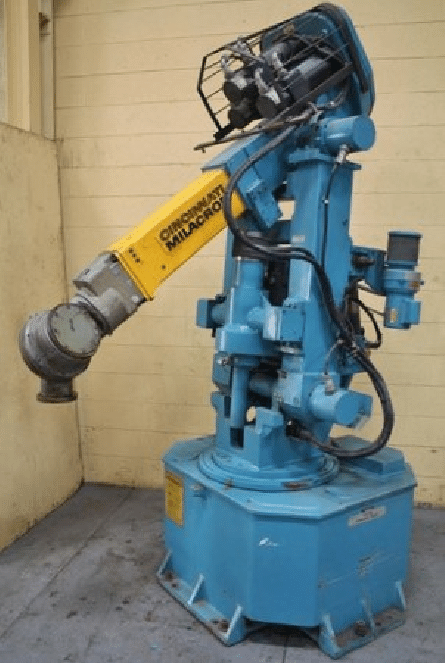
\includegraphics[width=55mm]{figs/T3_robot.png}
    \end{center}
    \caption{Robot Cincinnati Milacron T3}
    \label{fig:T3}
  \end{figure}
  
La tercera generación, o robots industriales (1978-1999), disponían de controladores específicos (ordenadores), siendo un punto clave en la caracterización de esta generación, además del surgimiento de nuevos lenguajes de programación para el control de los robots, la posibilidad de reprogramarlos y la inclusión parcial de la visión artificial \cite{Zamalloa17}. A finales de los años setenta y principios de los ochenta, otros avances científicos y técnicos contribuyeron a la difusión de los robots \cite{Gasparetto19}, que junto a que las empresas de todo el mundo invirtieron miles de millones de dólares en del mundo para automatizar tareas básicas en sus cadenas de montaje, supusieron que los robots poblaran muchos sectores industriales para automatizar una amplia variedad de actividades \cite{Zamalloa17}.\\ 

En 1978, Unimation diseñó y fabricó el robot PUMA. El PUMA (\textit{Programmable Universal Machine for Assembly}) fue considerado durante muchas décadas el arquetipo de los robots antropomórficos \cite{Gasparetto19}. Ese mismo año, el científico japonés Hiroshi Makino, de la Universidad de Yamanashi, propuso una nueva estructura cinemática. El robot con esta estructura se denominó SCARA (\textit{Selective Compliance Assembly Robot Arm})(ver Figura \ref{fig:Scara}), ya que su conformidad en la dirección horizontal resultó menor que la conformidad en la dirección vertical. Por esta razón, así como por la ligereza de la cadena cinemática (que permitía un controlador más sencillo y rápido), este robot era adecuado para ser empleado en tareas como el ensamblaje de objetos pequeños \cite{Makino80}.
  
  \begin{figure} [H]
    \begin{center}
      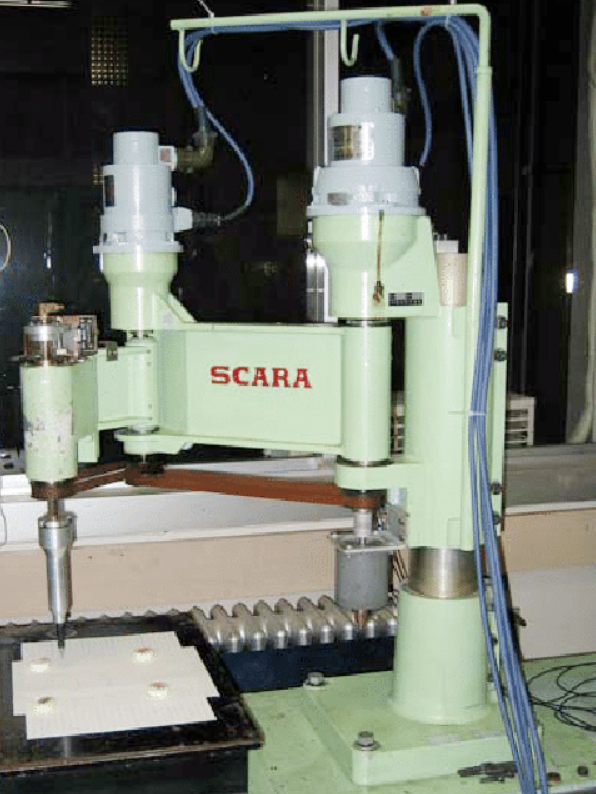
\includegraphics[width=45mm]{figs/Scara.png}
    \end{center}
    \caption{Uno de los primeros prototipos de robot SCARA}
    \label{fig:Scara}
  \end{figure}
  
Más tarde, en 1981, en la Universidad Carnegie-Mellon se desarrolló un robot de impulsión directa que utiliza motores eléctricos en las articulaciones, evitando la distorsión de las transmisiones mecánicas convencionales. En 1982, IBM introduce el robot de montaje industrial RS-1 que utiliza un brazo constituido por 3 dispositivos de deslizamiento \cite{Sanchez07b}. De la idea de emplear cadenas cinemáticas paralelas en lugar de las clásicas cadenas cinemáticas en serie, junto con la de crear un robot ligero capaz de moverse a gran velocidad, surgió el arquetipo del robot Delta (que apareció en 1992), concebido por el científico suizo Reymond Clavel en la Escuela Politécnica Federal de Lausana (EPFL) \cite{Clavel91}. En comparación con los robots en serie, los robots paralelos tienen un espacio de trabajo más pequeño, pero pueden funcionar a una velocidad mucho mayor, siendo la arquitectura cinemática ideal para los robots dedicados a operaciones de pick-and-place de alta velocidad. Basado en este tipo de estructura, unos años después, en 1998, ABB desarrolló el Flex-Picker (Figura \ref{fig:Flexpicker_ABB}, el robot de picking más rápido del mundo \cite{Gasparetto19}.\\
  
  \begin{figure} [H]
    \begin{center}
      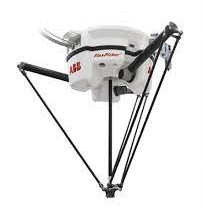
\includegraphics[width=45mm]{figs/flexpicker_ABB.jpeg}
    \end{center}
    \caption{Robot ABB IRB 360 Flexpicker}
    \label{fig:Flexpicker_ABB}
  \end{figure}
  
A partir de los años 2000, aparece la cuarta generación o robots inteligentes (2000-Actualidad), que se caracteriza por la inclusión de capacidades informáticas avanzadas, ya que los ordenadores no sólo trabajan con datos, si no también pueden realizar razonamientos lógicos y aprender, puesto que la Inteligencia Artificial comienza a ser incluida parcial y experimentalmente en estos robots. Los sensores son más sofisticados, y envían información al controlador y la analizan mediante estrategias de control complejas para que el robot pueda basar sus acciones en información sólida y fiable. Es en esta generación cuando se introducen los robots colaborativos \cite{Zamalloa17}.\\
  
Los requisitos de velocidad y peso de un robot han dado lugar a novedosos diseños cinemáticos y de transmisión. Desde el principio, la reducción de la masa y la inercia de las estructuras robóticas ha sido un objetivo primordial en el desarrollo de la robótica. El brazo humano, con una relación peso-carga de 1:1, se consideraba la referencia definitiva \cite{Siciliano16}. Con este objetivo se desarrollaron, gracias a la colaboración entre la empresa alemana KUKA y el Instituto de Robótica y Mecatrónica del Centro Aeroespacial Alemán (DLR), tres generaciones de robots ligeros, permitiendo a investigadores e ingenieros desarrollar nuevas aplicaciones de robótica industrial y de servicios con un rendimiento sin precedentes. En el año 2004, con motivo de Automática, la mayor exposición de robots del mundo, se presentó por primera vez la combinación entre el robot ligero del DLR y la controladora KUKA, denominado RoboAssistant, donde se permitió a los visitantes mover y programar manualmente el robot, haciendo la visión de un robot que asiste a un trabajador durante los procesos de producción evidente para los visitantes \cite{Bischoff10}. \\
  
  
Es en estos procesos de producción, donde la manipulación a dos manos puede ser crítica para tareas de ensamblaje complejas, manipulación simultánea
y procesamiento de piezas de trabajo o para la manipulación de objetos de gran tamaño, por lo que en 2005, MOTOMAN presenta el primer robot comercial para la manipulación sincronizada a dos manos \cite{Siciliano16} (ver Figura \ref{fig:MOTOMAN}).\\

  \begin{figure} [H]
    \begin{center}
      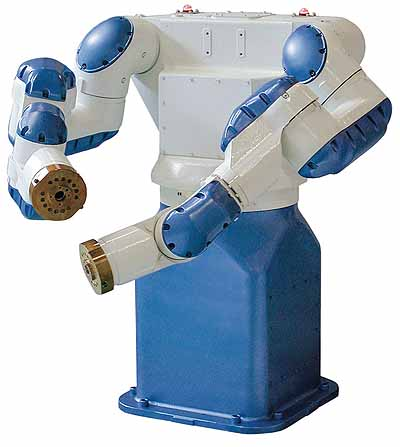
\includegraphics[width=55mm]{figs/MOTOMAN.jpg}
    \end{center}
    \caption{Robot Motoman DA-20}
    \label{fig:MOTOMAN}
  \end{figure}
  
Sin embargo, fue en el año 2006 cuando, tras haber estado trabajando en la búsqueda de vías para el desarrollo en serie del robot LWR3 del DLR, y tras una intensa cooperación entre KUKA y el DLR para transmitir a los desarrolladores de KUKA los conocimientos necesarios para para el desarrollo de brazos ligeros, componentes y electrónica integrada, cuando se toma la decisión de producir una primera pequeña serie del robot ligero del KUKA LWR3 \cite{Bischoff10}, tal y como muestra la Figura \ref{fig:Lightweight Robot (LWR)}.
  
  \begin{figure}[h!]
    \begin{center}
      \subcapcentertrue
      \subfigure[RoboAssistant en Automatica 2004]{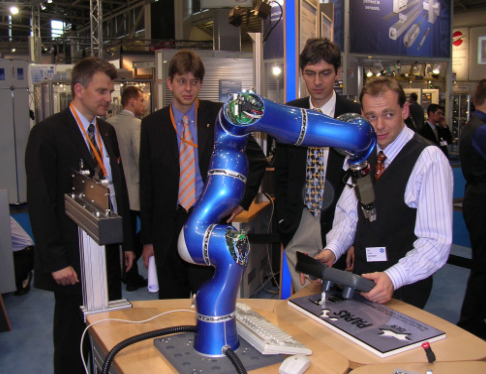
\includegraphics[width=65mm]{figs/RoboAssistant.png}}
      \hspace{2mm}
      \subfigure[Robot KUKA LWR3 con controladora (2006)]{\includegraphics[width=55mm]{figs/Kuka_lightweightrobot_2006.png}}
    \end{center}
    \caption{LWR3}
    \label{fig:Lightweight Robot (LWR)}
  \end{figure}
  
A principios de 2007, dos estudiantes de doctorado de la Universidad de Standford, Keenan Wyrobek y Eric Bergerlas, pusieron las primeras piezas de lo que eventualmente se convertiría en ROS (Robot Operating System). Uno de los preceptos principales que se tuvo en cuenta para la creación de este sistema operativo para robots fue el de crear un sistema que permitiese al máximo posible la reutilización de código, dando soporte a distintos tipos de robots y de aplicaciones. Esto resultó en la incorporación de ROS en una sorprendentemente amplia variedad de robots, extendiéndose incluso a dominios más allá de la comunidad académica de investigación a la que se dirigió inicialmente. Los años siguientes superaron todas las expectativas debido a que los avances en el ámbito de la robótica se compartieron de manera reproducible en ROS, y la Open Source Robotics Foundation (OSRF) se convirtió en el administrador principal de ROS en 2014. Con el objetivo de atender de manera más efectiva las demandas de una comunidad ROS más extensa y abordar sus nuevos escenarios de aplicación, la OSRF se dedicó a desarrollar ROS2 como un conjunto de paquetes paralelos que pudieran ser instalados junto a ROS1 (la versión original de ROS que nació en el año 2010)(Figura \ref{fig:PR_ROS}) y ser compatibles entre sí. Además, la popularidad de ROS ha seguido creciendo en la industria con el apoyo de proyectos como ROS-Industrial (ROS-I), una iniciativa de código abierto que extiende las capacidades avanzadas de ROS a hardware y aplicaciones industriales relevantes. \cite{Suarez22}.\\
  
  \begin{figure}[H]
    \begin{center}
      \subcapcentertrue
      \subfigure[Robot PR1]{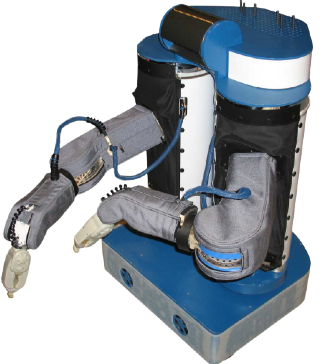
\includegraphics[width=52mm]{figs/PR1.png}}
      \hspace{2mm}
      \subfigure[Robot PR2]{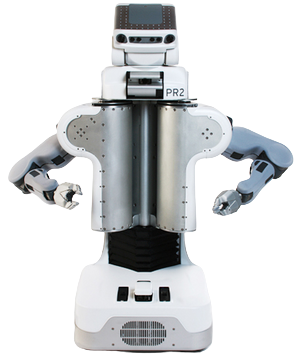
\includegraphics[width=50mm]{figs/PR2.png}}
    \end{center}
    \caption{Robots utilizados para el desarrollo de ROS}
    \label{fig:PR_ROS}
  \end{figure}
  
  
  \begin{figure} [H]
    \begin{center}
      
\includegraphics[width=55mm]{figs/ROS_logo.png}
    \end{center}
    \caption{Logo de ROS}
    \label{fig:ROS}
  \end{figure}
  
  \pagebreak
  
En el año 2008 se entrega el primer robot colaborativo o cobot, el UR5 de Universal Robots \footnote{\url{https://www.universal-robots.com/es/}} (ver Figura \ref{fig:UR5}), considerado como uno de los logros tecnológicos más significativos de la década en la comunidad robótica. El brazo robótico es pionero en la programación 3D fácil de usar pero sofisticada, con una interfaz de usuario intuitiva que permite a cualquier persona configurarlo y utilizarlo de forma rápida. Esta empresa, fundada en el año 2005 por Esteben Østergaard, Kasper Støy y Kristian Kassow tras conocerse en la Universidad de Dinamarca, surgió con el objetivo de hacer que la robótica sea accesible para las pequeñas y medianas empresas \footnote{\url{https://www.universal-robots.com/es/acerca-de-universal-robots/nuestra-historia/}}.\\
  
Esben H. Østergaard, Director de Tecnología y cofundador de Universal Robots, tomó el trabajo original de Peskhin y Colgate, dos investigadores de la empresa automovilística Ford de los años 90, que decidieron crear un nuevo robot industrial, más pequeño y ágil que los tradicionales, que saliera de su jaula para colaborar estrechamente con el ser humano en las tareas de calidad y personalización de los productos, sin embargo, no fueron capaces, puesto que el problema estaba en la relación entre seguridad y rendimiento, ya que el aumento de la primera reducía el de la segunda. Østergaard consiguió diseñar un sistema de seguridad y control para el cobot que lo bloquea en caso de colisión con el operario. Como recuerda el propio Østergaard, la seguridad era la clave con la que la robótica colaborativa podía entrar en el escenario industrial. Así se creó un robot capaz de operar en espacios confinados, en estrecho contacto con humanos, y sin instalar costosas barreras de seguridad \cite{Cusano22}.
  
  \begin{figure} [h!]
    \begin{center}
      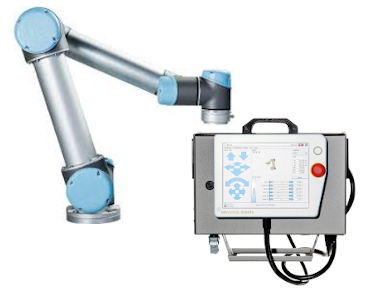
\includegraphics[width=75mm]{figs/UR5_controller.png}
    \end{center}
    \caption{UR5 con su controladora}
    \label{fig:UR5}
  \end{figure}
  
  \pagebreak
  
Más tarde, en 2018, Universal Robots presenta los robots colaborativos e-Series, que se pueden ver en la Figura \ref{fig:UR_e-series}, que incluían avances tecnológicos que permitían un desarrollo más rápido para una mayor variedad de aplicaciones, ofrecía una programación más sencilla y seguía las normas de seguridad ISO más actuales y recientes \footnote{\url{https://www.universal-robots.com/es/acerca-de-universal-robots/nuestra-historia/}}.
 
  \begin{figure}[H]
    \begin{center}
      \subcapcentertrue
      \subfigure[UR presenta los  nuevos e-Series en Automatica 2018]{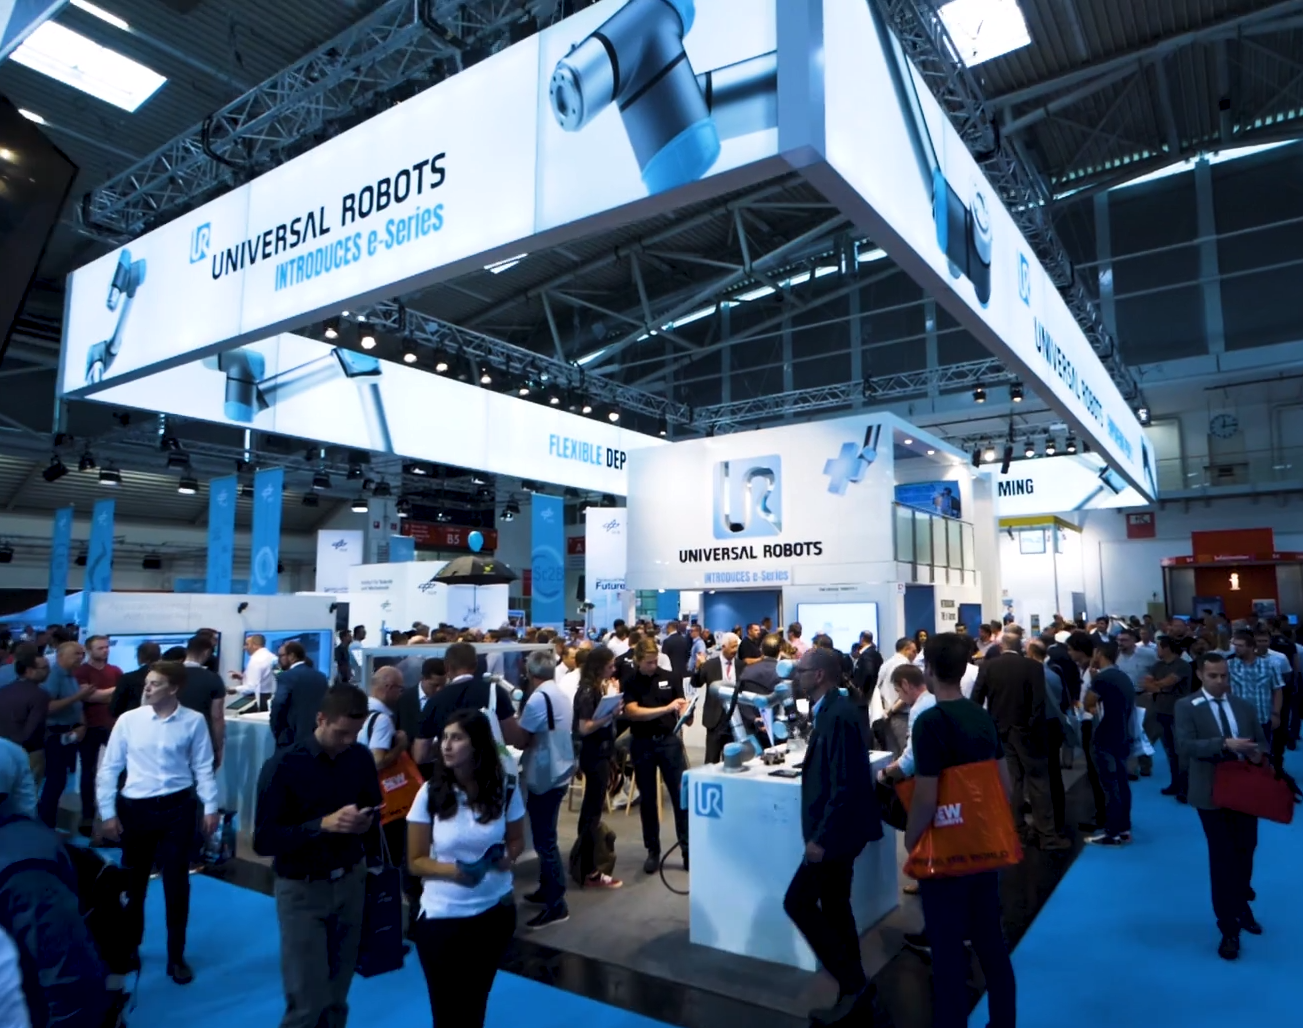
\includegraphics[width=72mm]{figs/UR Automatica 2018.png}}
      \hspace{2mm}
      \subfigure[UR e-Series]{\includegraphics[width=65mm]{figs/UR e-series.jpg}}
    \end{center}
    \caption{Universal Robots e-Series}
    \label{fig:UR_e-Series}
  \end{figure}
	  
Esta cuarta generación de robótica industrial ha establecido un sólido punto de partida para una continua revolución en el campo de la automatización. 
Es esencial destacar que varios de los modelos de robots mencionados previamente han seguido evolucionando y mejorando con el tiempo, siendo fruto de estas mejoras, la comercialización de nuevos modelos y series. 
Debido a que la tecnología se encuentra en constante desarrollo y a la colaboración cada vez más estrecha entre humanos y robots, el futuro de la robótica industrial promete seguir transformando radicalmente nuestros métodos de trabajo y producción, abriendo así nuevas oportunidades y desafiando constantemente los límites de lo que podemos lograr en la automatización industrial, así como en los otros dos grandes grupos de la robótica, como la robótica de servicio y la robótica médica.

\pagebreak
   
\subsection{Robots de servicio}
\label{sec:robot_servicio}

Se define robot de servicio como un robot que realiza tareas útiles para las personas o los equipos, incluyendo en esta la manipulación o el servicio de artículos, el transporte, el apoyo físico, la orientación o información, el aseo personal, la cocina y la manipulación de alimentos y la limpieza en el ámbito personal; y la inspección, vigilancia, manipulación de objetos, transporte de personas, orientación o información, cocina y manipulación de alimentos y limpieza en el ámbito profesional \cite{ISO8373}.\\

Su historia se remonta a la década de 1960, cuando surgieron los primeros intentos de crear robots para ayudar en tareas domésticas y de atención al cliente. Uno de los precursores de estos robots de servicio en 1968 fue el robot Shakey, desarrollado por el Laboratorio de Investigación de Inteligencia Artificial de Stanford (Stanford Research Institute, SRI). Shakey (ver en Figura \ref{fig:shakey}), provisto de múltiples sensores y medios para desplazarse por el suelo, además de control remoto por radio \cite{Sanchez07b}, podía realizar tareas de planificación, búsqueda de rutas y reordenación de objetos sencillos, siendo el primer robot móvil con capacidad para percibir y razonar sobre su entorno \footnote{\url{https://www.sri.com/hoi/shakey-the-robot/}}. 

  \begin{figure} [H]
    \begin{center}
      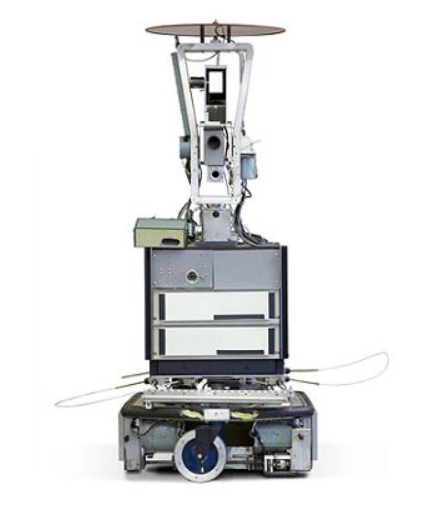
\includegraphics[width=65mm]{figs/Shakey.png}
    \end{center}
    \caption{Robot Shakey}
    \label{fig:shakey}
  \end{figure}
  
  \pagebreak
   
Sin embargo, fue a mediados de los años 80 cuando en los laboratorios y centros de investigación dedicados a la robótica se trató de revitalizar la importancia de los robots en nuestra sociedad, planteando las ventajas que el uso del robot podía traer en tareas en las que el ser humano asumía riesgos o en las que las capacidades de aquel estaban limitadas por factores como la fuerza o la precisión necesaria. Fue precisamente al entenderse que estas nuevas aplicaciones de la robótica no tenían un uso industrial con el objetivo de fabricar bienes, sino que se trataba de un empleo para desarrollar tareas para las personas, cuando se catalogaron como aplicaciones en el sector servicios \cite{Barrientos02}(ver ejemplos en la Figura \ref{fig:Robots_servicio}).\\

En la práctica, las actuales y potenciales aplicaciones no industriales de los robots son tan variadas y diferentes que se dificulta su catalogación \cite{Barrientos02}; sin embargo, existen ciertas características especiales en estos robots de servicio que los hacen diferentes de los robots industriales \cite{Aracil08}, y los caracterizan para llevar a cabo estas tareas para las personas, siendo las principales características estos tres atributos de diseño: representación, antropomorfismo y orientación a la tarea, es decir, los robots de servicio pueden tener una representación física (por ejemplo, Pepper) o tener una representación únicamente virtual (por ejemplo, Alexa, ya que el software de IA virtual que funciona de forma autónoma y aprende con el tiempo también puede clasificarse como robot de servicio), diseñarse como humanoides (es decir, antropomorfos) simulando una apariencia humana o como no humanoides (por ejemplo, el robot de limpieza Roomba de iRobot \footnote{\url{https://www.irobot.es/}} (Figura \ref{fig:roomba}), y pueden realizar tareas cognitivo-analíticas gracias a la potencia informática subyacente o tareas emocionales-sociales (por ejemplo, robots de recepción) \cite{Wirtz18}.\\

 \begin{figure}[H]
    \begin{center}
      \subcapcentertrue
      \subfigure[Alexa]{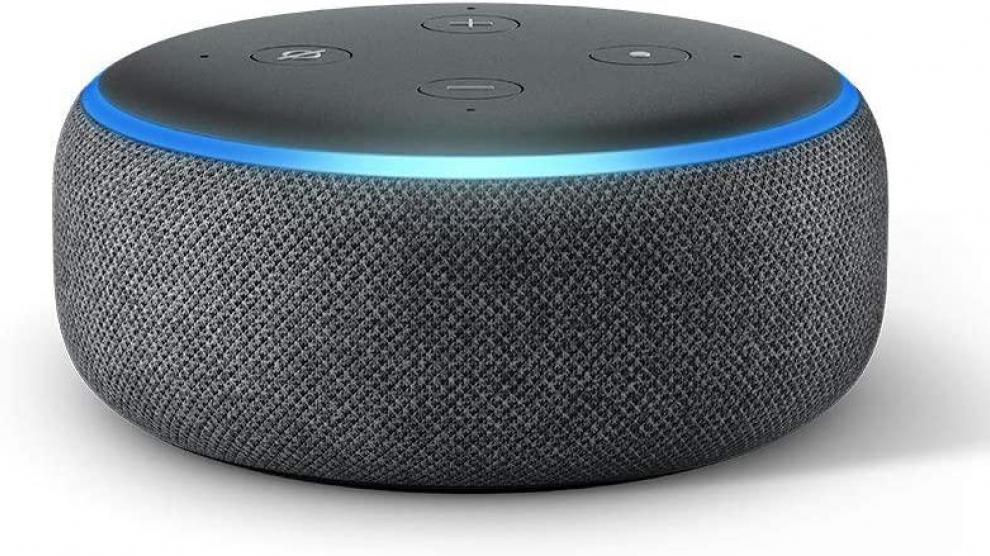
\includegraphics[width=45mm]{figs/Alexa.jpeg}}
      \hspace{2mm}
      \subfigure[Pepper]{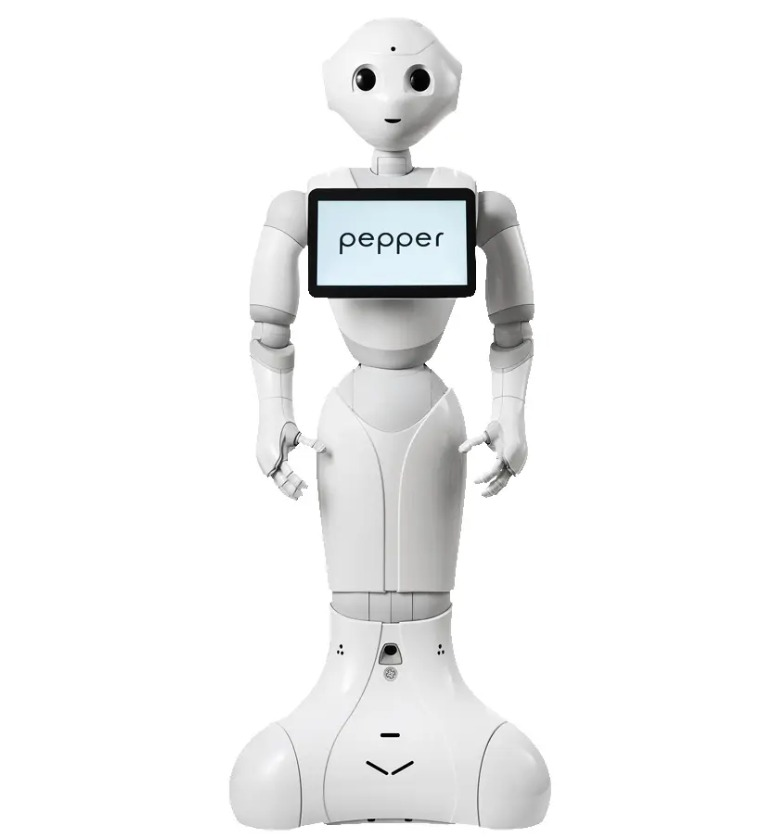
\includegraphics[width=45mm]{figs/Pepper.jpeg}}
      \hspace{2mm}
      \subfigure[Sophia]{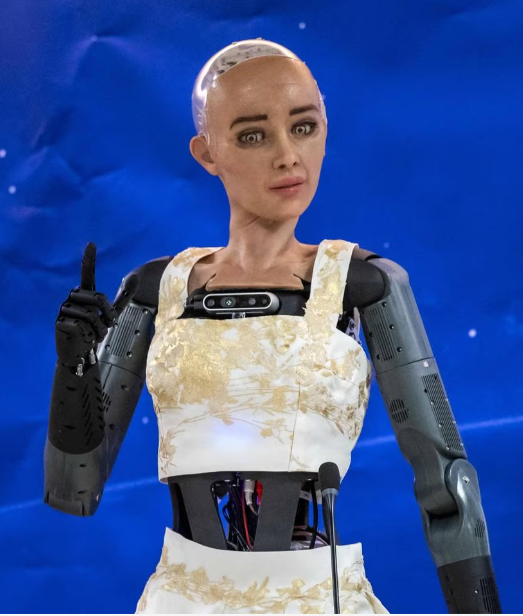
\includegraphics[width=38mm]{figs/Sophia.png}}
    \end{center}
    \caption{Robots de servicio}
    \label{fig:Robots_servicio}
  \end{figure}

Tratando de establecer una división de los robots de servicio, la norma ISO 8373:2012, así como la Federación Internacional de Robótica o IFR, propuso clasificarles en diferentes categorías según su función y aplicación en robots para uso doméstico y personal y robots de servicio destinados a un uso profesional \cite{Gonzalez21}, siendo las aplicaciones más importantes las siguientes:

\begin{itemize}
 \item \textit{Limpieza:} Suelen estar equipados con sensores y tecnología de navegación que les permite moverse de manera autónoma por el espacio, detectar obstáculos y llevar a cabo actividades de limpieza de manera eficiente. 
 
 \begin{figure} [H]
  \begin{center}
    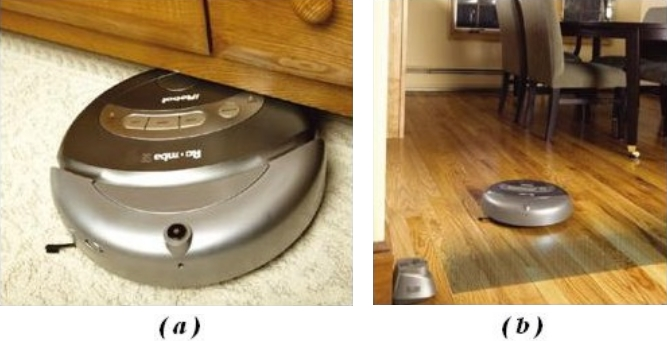
\includegraphics[width=90mm]{figs/roomba}
  \end{center}
  \caption{Robot aspirador Roomba de iRobot}
  \label{fig:roomba}
 \end{figure}
 
 \item \textit{Inspección y mantenimiento:} Son máquinas diseñadas para llevar a cabo tareas de supervisión, evaluación y mantenimiento en entornos de infraestructura o áreas de difícil acceso. Estos robots suele ser máquinas autónomas o teleoperadas equipadas con sensores, cámaras y herramientas especializadas que les permiten evaluar, reparar y mantener equipos, estructuras y sistemas en entornos desafiantes o peligrosos. 
 
 \begin{figure}[H]
    \begin{center}
      \subcapcentertrue
      \subfigure[Spot de Boston Dynamics]{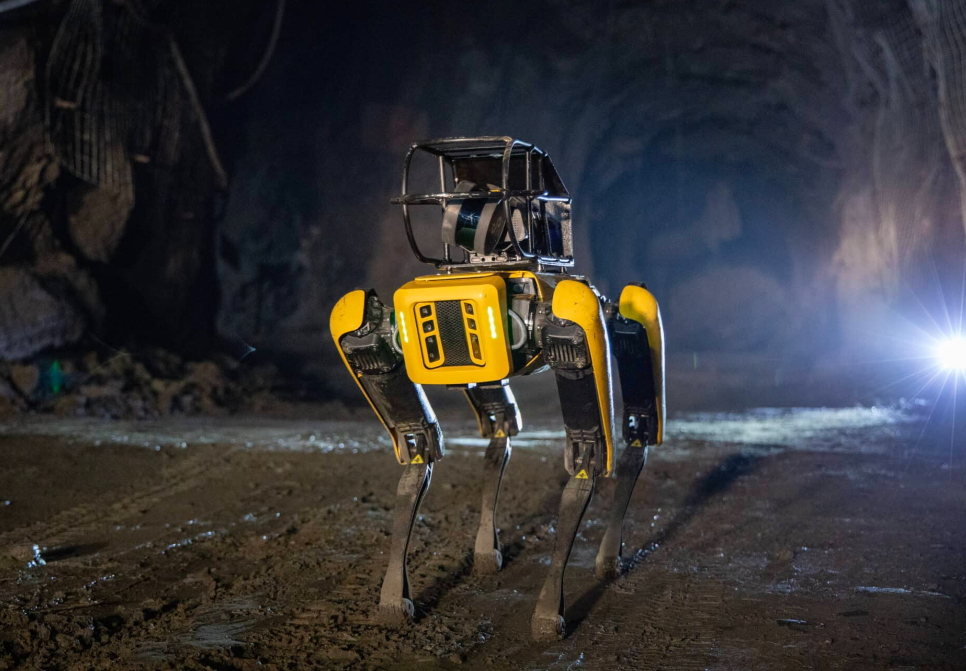
\includegraphics[width=60mm]{figs/Spot.png}}
      \hspace{2mm}
      \subfigure[ROBTET, robot para el mantenimiento de líneas de alta tensión]{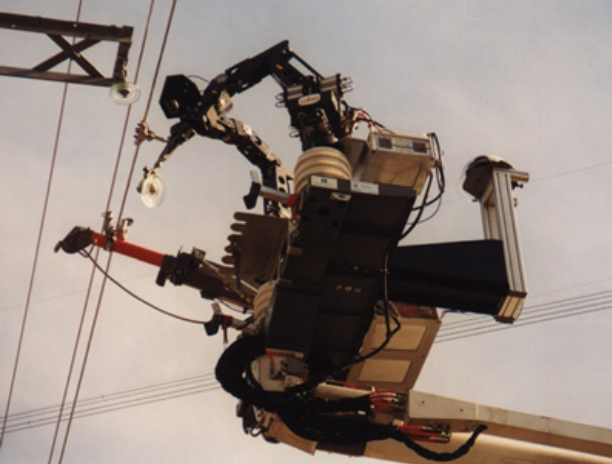
\includegraphics[width=55mm]{figs/ROBTET.png}}
    \end{center}
    \caption{Robots de inspección y mantenimiento}
    \label{fig:Robots de inspección y mantenimiento}
  \end{figure}
 
 
 \item \textit{Educación:} Aquellos robots utilizados en educación son robots diseñados para facilitar el aprendizaje y la enseñanza en los diferentes niveles educativos. Estos robots pueden ser utilizados en aulas, bibliotecas y entornos de aprendizaje para ayudar a los estudiantes a adquirir habilidades, fomentar la creatividad y brindar experiencias educativas interactivas.\\
 
 \begin{figure}[H]
    \begin{center}
      \subcapcentertrue
      \subfigure[Robot NAO]{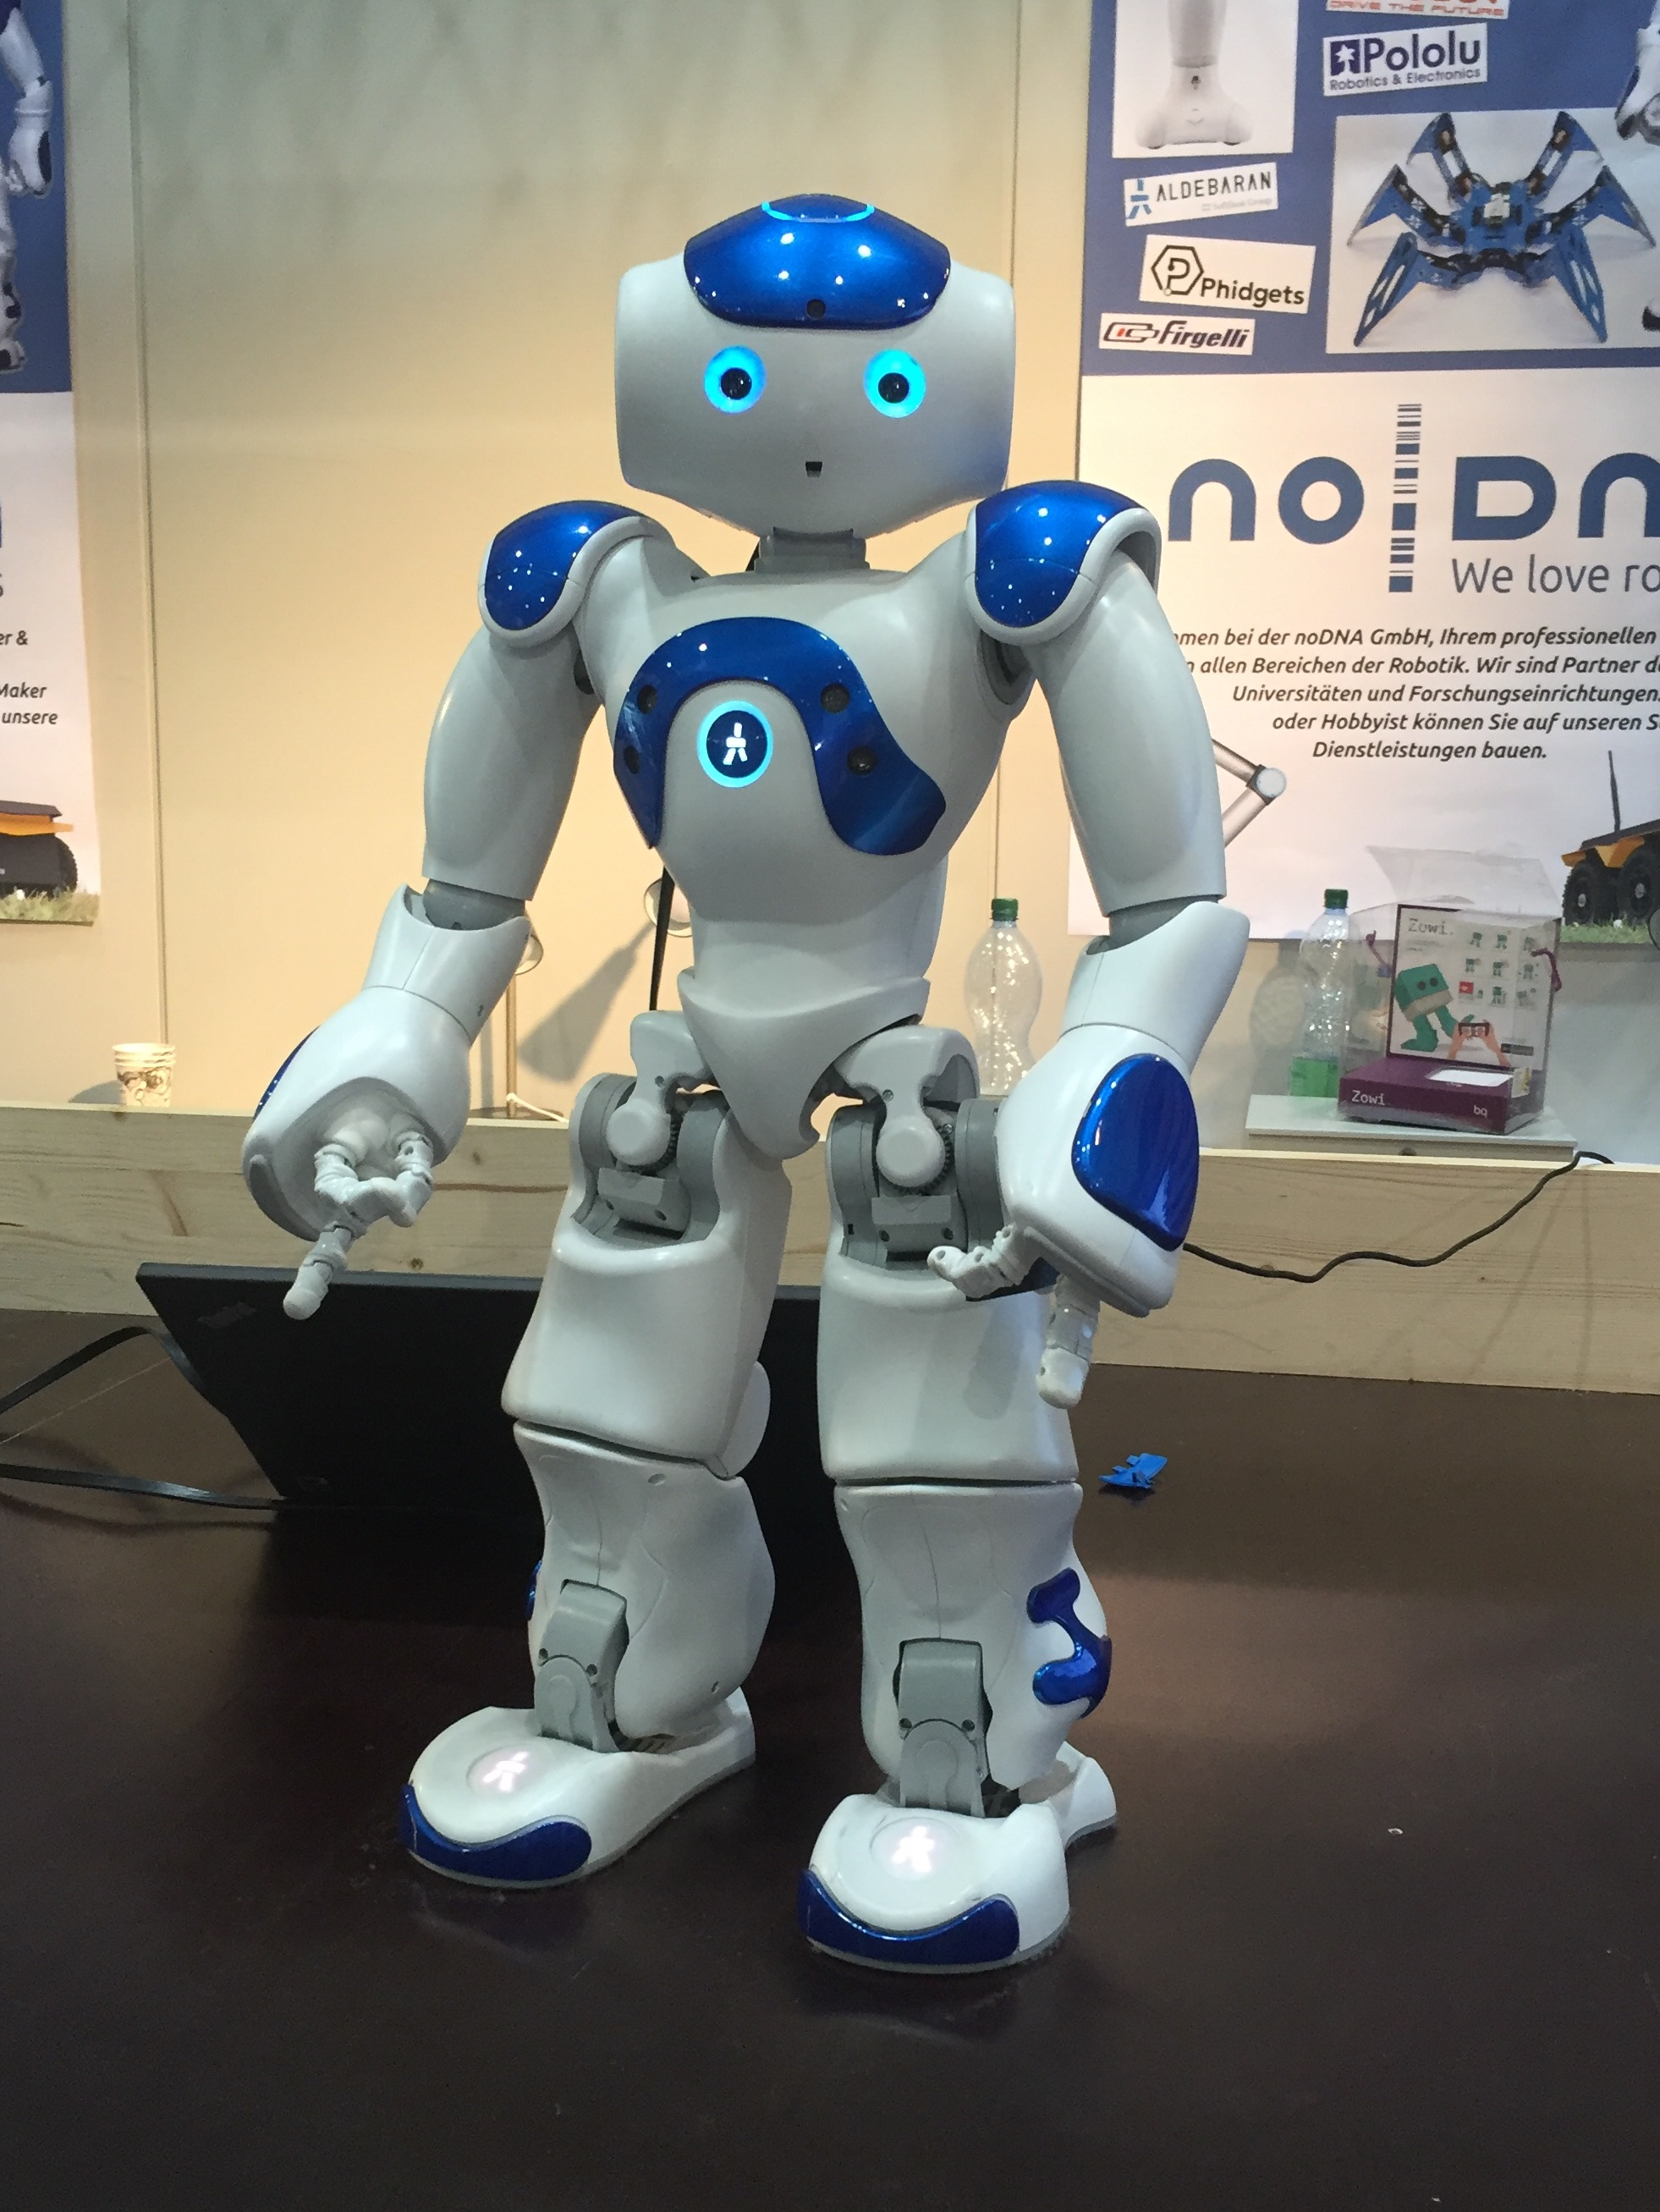
\includegraphics[width=40mm]{figs/Robot NAO.jpg}}
      \hspace{2mm}
      \subfigure[Turtlebot 4]{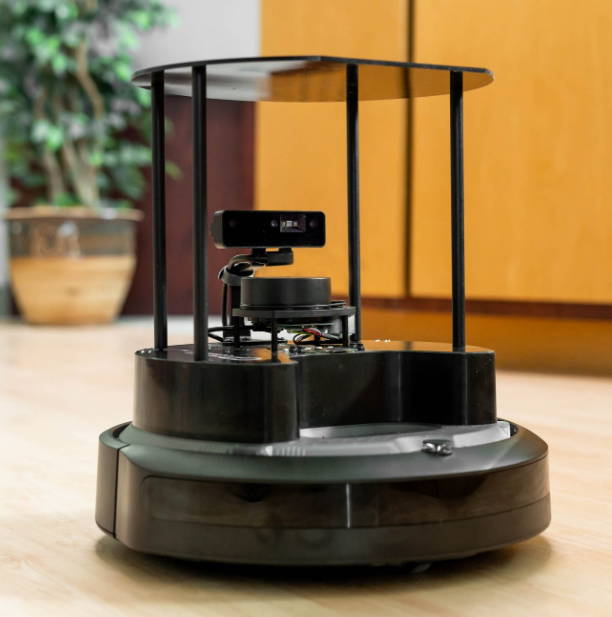
\includegraphics[width=53mm]{figs/Turtlebot 4.png}}
    \end{center}
    \caption{Robots de educación}
    \label{fig:Robots de educación}
  \end{figure}
 
 \item \textit{Logística:} Los robots de servicio utilizados en logística son robots diseñados para llevar a cabo tareas relacionadas con la gestión y el movimiento de mercancías y productos en entornos de almacenamiento, distribución y transporte. Estos robots desempeñan un papel fundamental en la optimización de la cadena de suministro, mejorando la eficiencia y la precisión en la manipulación de productos. Un ejemplo del posible uso de estos robots en el sector agrícola, es la primera granja vertical de interior del mundo en Estados Unidos, que producirá 18 millones de kilogramos de fresas al año, marcando un hito en la agricultura moderna, y demostrando que la automatización e integración de la robótica en este tipo de granjas verticales puede transformar la producción y recolección de alimentos a gran escala \cite{EcoInventos24}.
 
 \begin{figure} [H]
  \begin{center}
    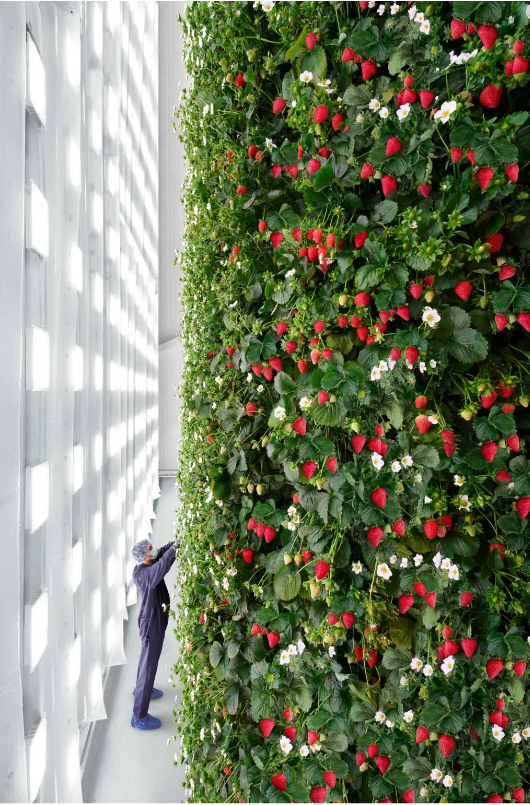
\includegraphics[width=70mm]{figs/agricultura vertical 1.png}
  \end{center}
  \caption{Agricultura vertical}
  \label{fig:agricultura_vertical}
 \end{figure}
 
Por otro lado, dentro de los robots de logística empleados para el movimiento de mercancías, se pueden distinguir dos grandes grupos: Vehículos Guiados Automáticos (AGV) y Robots Móviles Autónomos (AMR). La principal diferencia entre los AMR y los AGV radica en la capacidad de adaptación y autonomía, ya que los AMR son altamente flexibles, autónomos y versátiles, con capacidades autónomas avanzadas que les permiten ajustarse rápidamente a cambios en los entornos de trabajo, mientras que los AGV siguen rutas predefinidas y son adecuados para tareas de transporte predecibles en entornos más controlados.
 
 \begin{figure}[H]
    \begin{center}
      \subcapcentertrue
      \subfigure[AGV Robots Kiva de Amazon]{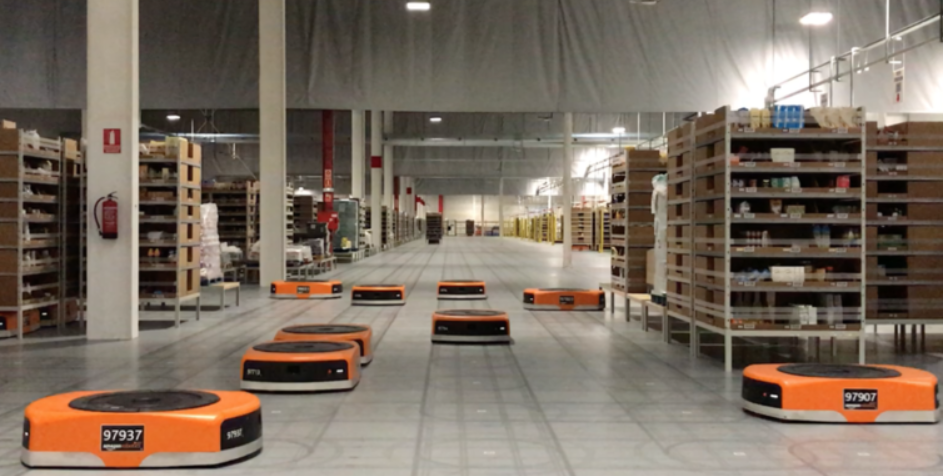
\includegraphics[width=67mm]{figs/AGV Amazon.png}}
      \hspace{2mm}
      \subfigure[AMRs de MiR]{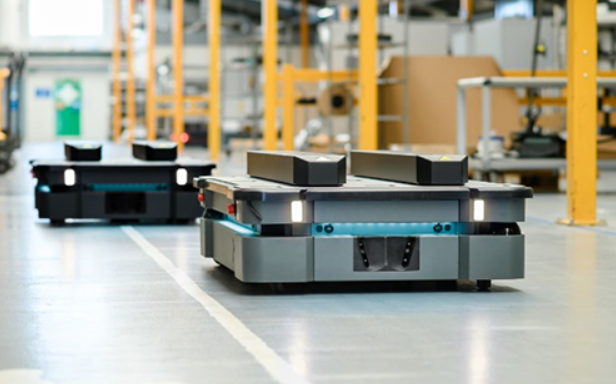
\includegraphics[width=55mm]{figs/MiR.png}}
    \end{center}
    \caption{Robots de logística}
    \label{fig:Robots de logística}
  \end{figure}
  
 \item \textit{Entretenimiento:} Son robots diseñados específicamente para proporcionar experiencias lúdicas y de entretenimiento a las personas. Estos robots se utilizan en una variedad de contextos, siendo máquinas robóticas diseñadas para interactuar con el público. 
 
  \begin{figure}[H]
    \begin{center}
      \subcapcentertrue
      \subfigure[SONY Aibo]{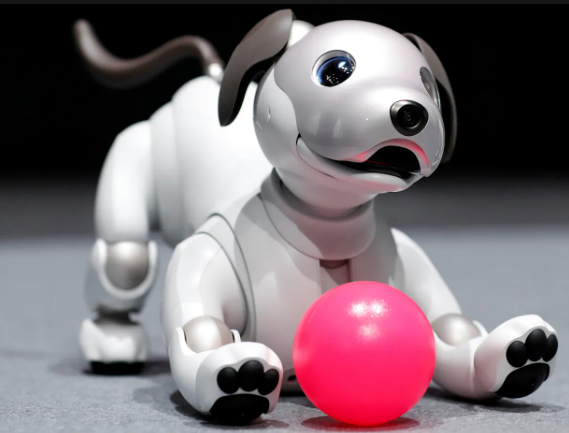
\includegraphics[width=50mm]{figs/SONY Aibo.png}}
      \hspace{2mm}
      \subfigure[Dron DJI Spark]{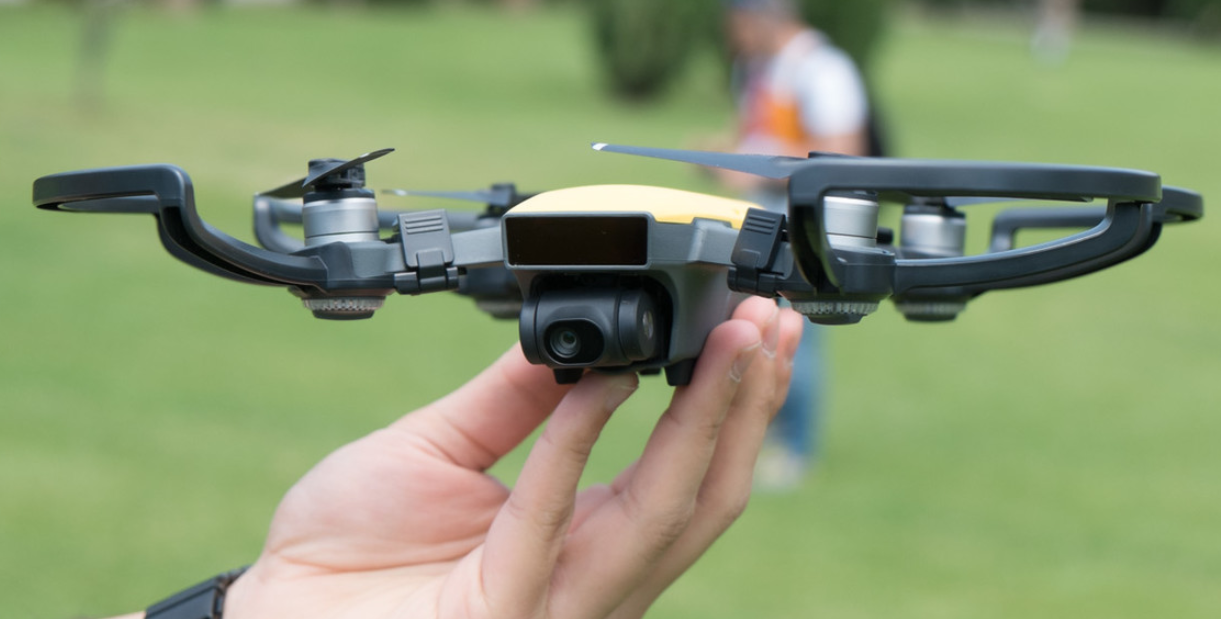
\includegraphics[width=76mm]{figs/Dron DJI Spark.png}}
    \end{center}
    \caption{Robots de entretenimiento}
    \label{fig:Robots_entretenimiento}
  \end{figure}
   
\end{itemize}

La robótica de servicio representa una revolución en la asistencia y el apoyo a diversas industrias, desde la logística hasta la atención al cliente en el comercio minorista. Sin embargo, su impacto va más allá, extendiéndose hasta la atención médica. En este contexto, la robótica médica emerge como una vanguardia tecnológica que fusiona la innovación robótica con la medicina moderna para ofrecer soluciones innovadoras en diagnóstico, tratamiento y rehabilitación, demostrando su potencial para revolucionar la forma en que brindamos y recibimos atención médica.
\pagebreak
 
\subsection{Robot Médico}
\label{sec:robotica_industrial} 

Se define \textit{robot médico} como aquellos dispositivos electromecánicos que desempeñan parcial o totalmente algunas funciones de los seres humanos o de sus órganos al resolver problemas médicos, ayudando a mejorar la asistencia al paciente y los resultados, a la vez que aumenta la eficiencia operativa \cite{Kraevsky10}.\\

Los robots médicos se desarrollaron por primera vez hace poco más de tres décadas para permitir a los cirujanos operar a sus pacientes a distancia o con mayor precisión. A finales de los años noventa, había 2 tipos de telemanipuladores quirúrgicos aprobados por la Administración de Alimentos y Medicamentos de los Estados Unidos (FDA): el Zeus y el da Vinci (Figura \ref{fig:RobotDaVinci}), introducido en 1998-1999, que permitía aumentar la precisión de las cirugías mínimamente invasivas (CMI) \cite{Romero20}.\\

\begin{figure} [H]
    \begin{center}
      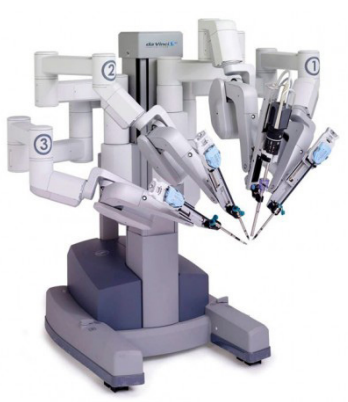
\includegraphics[width=10cm]{figs/Robot Da Vinci.png}
    \end{center}
    \caption{Robot Da Vinci}
    \label{fig:RobotDaVinci}
\end{figure}

Las primeras aplicaciones fueron en los campos de neurocirugía y cirugía ortopédica, siendo la cirugía donde mayor impacto han tenido los robots médicos. A medida que se ha hecho patente la aceptación de los robots quirúrgicos por nuestros sistemas sanitarios, los investigadores en robótica han ido centrando cada vez más su atención en cómo podría ser la próxima generación de robots médicos. Su atención no se limita a los robots quirúrgicos, y también se están investigando otras áreas de la medicina, como los robots para realizar rehabilitación física con pacientes con discapacidades motores, como el exoesqueleto Ekso Bionics, robots de telepresencia para la interacción del paciente con el personal sanitario externo, como el robot RP-VITA, automatización de farmacias, robots para desinfectar clínicas, etc. \cite{Dupont21}\\

 \begin{figure}[H]
    \begin{center}
      \subcapcentertrue
      \subfigure[Exoesqueleto Ekso Bionics]{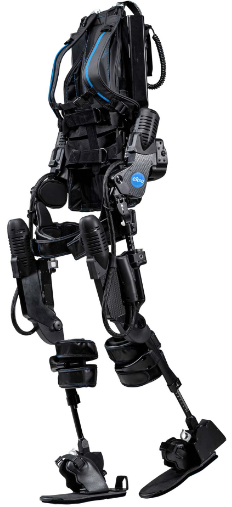
\includegraphics[width=35mm]{figs/Ekso Bionics.png}}
      \hspace{20mm}
      \subfigure[Robot RP-VITA]{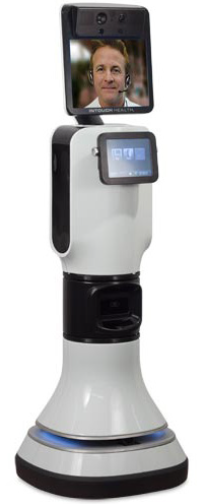
\includegraphics[width=35mm]{figs/RP Vita.png}}
    \end{center}
    \caption{Robots médicos}
    \label{fig:Robots_medicos}
  \end{figure}

El rápido crecimiento de la robótica médica se debe a una combinación de mejoras tecnológicas (motores, materiales y teoría de control), los avances en imagen médica (mayor resolución, resonancia magnética y ecografía 3D) y una mayor aceptación por cirujanos y pacientes de los procedimientos laparoscópicos y la asistencia robótica \cite{Beasley12}, convirtiéndose en un campo interdisciplinario que abarca desde cirugía asistida por robots hasta sistemas de diagnóstico de vanguardia. Gran parte de su éxito radica en la integración de tecnologías avanzadas, como la inteligencia y la visión artificial. Estas disciplinas están redefiniendo la forma en que los robots médicos pueden interactuar con el entorno, interpretar datos y, en última instancia, mejorar los resultados en la atención médica. A continuación, explicaremos el impacto que la inteligencia y la visión artificial están teniendo en la robótica, y las capacidades y oportunidades que estas presentan en una inmensa variedad de aplicaciones.

\pagebreak

\section{Inteligencia Artificial}
\label{sec:IA} 

La Inteligencia Artificial (IA) es un área de la ciencia de gran interés por ser un área multidisciplinaria donde se realizan sistemas que tratan de hacer tareas y resolver problemas como lo hace un humano;así mismo, trata de simular de manera artificial las formas de pensamiento y de trabajar del cerebro para la toma de decisiones \cite{Ponce14}.\\

El origen del concepto y de los criterios de desarrollo de la IA se remontan al año 1936, con el matemático inglés Alan Turing, quien definió una máquina abstracta, la Máquina de Turing, un modelo matemático que consiste en un autómata capaz de implementar cualquier problema matemático expresado por medio de un algoritmo, que sirvió de base de la noción de algoritmo y la definición de clase de problemas deducibles \cite{Hardy01}, y quien intuyó la importancia que jugaría el aprendizaje automático en el desarrollo de la IA al afirmar que, en lugar de intentar emular mediante una máquina la mente de un adulto, quizá sería más factible intentar emular la mente de un niño y luego someter a la máquina a un proceso de aprendizaje que diera lugar a un desarrollo cognitivo de dicha mente hasta alcanzar el equivalente de una mente adulta, lo que actualmente se conoce como robótica de desarrollo \cite{Gonzalez17}, mientras que el apelativo Inteligencia Artificial se debe a John McCarthy, quien organizó una conferencia en el Darmouth College (Estados Unidos) en agosto de 1956, para discutir sobre la posibilidad de construir máquinas "inteligentes". Como resultado de esta reunión, se establecieron los primeras bases sobre la inteligencia de los computadores \cite{Ponce14}. \\

La historia de la IA ha sido testigo de ciclos caracterizados por la introducción de nuevos y creativos enfoques y de un sistemático perfeccionamiento de los mejores. Estos ciclos de avance y desafío continúan moldeando su evolución y prometen un futuro emocionante y lleno de posibilidades.\\

Dentro de las diversas formas de clasificar la IA, existe una clasificación de los modelos de Inteligencia Artificial tal y como se muestra en la Figura \ref{fig:ModelosInteligencia}), que se basa en el objetivo y la forma en que trabaja el sistema: sistemas que piensan como humanos, sistemas que actúan como humanos, sistemas que piensan racionalmente, y sistemas actuantes racionales. Esta clasificación de manera inicial se veía como clases independientes, sin embargo, en la actualidad los sistemas mezclan características de ellas. \cite{Ponce14} \\

\begin{figure} [h!]
    \begin{center}
      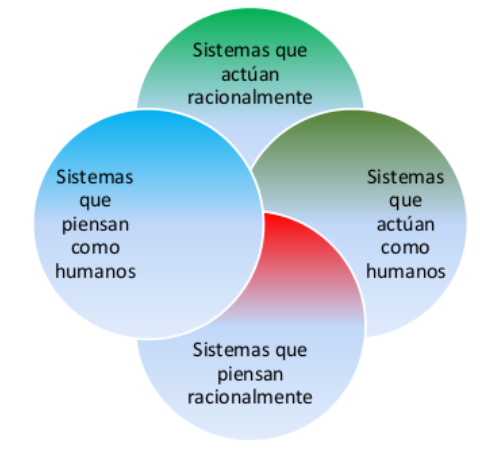
\includegraphics[width=9cm]{figs/Modelos de inteligencia.png}
    \end{center}
    \caption{Modelos de inteligencia}
    \label{fig:ModelosInteligencia}
\end{figure}

La clasificación de los modelos de IA tiene un impacto significativo en las aplicaciones de la IA, ya que determina cómo se desarrollan y aplican los sistemas de inteligencia artificial en una amplia gama de campos, contribuyendo así a la mejora de la eficiencia y la innovación en muchas industrias donde se han ido desarrollando diferentes herramientas propias y aplicaciones, dando lugar a multitud de ramas que parten de la IA. Una de las ramas más fascinantes y prometedoras de la inteligencia artificial es la visión artificial, que busca dotar a las máquinas de la capacidad de interpretar y comprender el mundo visual que les rodea. Esta sección del capítulo de introducción se centra en la importancia de la IA y su intersección con la visión artificial, explorando cómo estas disciplinas se fusionan para mejorar la percepción y la comprensión de imágenes y vídeos.

\pagebreak

\section{Visión Artificial}
\label{sec:VA} 

La visión artificial se define como la ciencia de programar un ordenador para procesar imágenes o vídeos e incluso entenderlos \cite{Culjak12}. 

En \cite{Bradski08} explica cómo es la transformación de datos desde un fotograma o vídeo cámara hasta lo que puede ser una decisión o una nueva representación \cite{Alvear17}. Para ello, la imagen percibida pasa por los procesos de obtención, caracterización e interpretación de información de imágenes, y estos procesos, pueden ser subdivididos a su vez en \cite{Santillan15}:\\

\begin{table} [h!]
  \begin{center}
      \includegraphics[width=16cm, height=8cm]{figs/Procesos de la visión artificial.png}
  \end{center}
  \caption{Procesos de la visión artificial}
  \label{cuadro:procesos_VA}
\end{table}

\begin{enumerate}
 \item \textit{Captura:} La captura o digitalización es el proceso en el que se obtiene una imagen digital a partir de una imagen analógica a través de un dispositivo para que pueda ser manipulada por un ordenador. Esta imagen estará representada como una matriz de números (píxeles) \cite{Martinez22}.
 
 \item \textit{Pre-procesamiento:} En esta fase, se incorporan métodos destinados a restaurar las imágenes capturadas, dado que es factible que las imágenes experimenten deterioro, como la disminución de su claridad o la presencia de ruido. Esta etapa tiene como objetivo corregir estos problemas mediante procedimientos como la eliminación de ruido o la mejora del contraste y la nitidez.
 
 \item \textit{Segmentación:} La segmentación consiste en dividir una imagen en regiones o componentes más pequeños (grupo de píxeles) con el objetivo de identificar y aislar objetos o áreas de interés dentro de la imagen. El propósito principal es simplificar y organizar la información visual contenida en la imagen para que sea más fácil de analizar, comprender y procesar por ordenador.

 \item \textit{Descripción:} Es el proceso que obtiene características relevantes para poder diferenciar un tipo de objeto de otro, pudiendo ser externas, como la forma, el perímetro o el rectángulo mínimo que contiene la región; o internas, como el área o el centro de gravedad, entre otros \cite{Santillan15}. 
 
 \item \textit{Reconocimiento (clasificación):} Esta fase se centra en identificar y asignar etiquetas o categorías a objetos o patrones previamente segmentados en una imagen o secuencia de imágenes. El proceso de reconocimiento implica el uso de algoritmos y técnicas de aprendizaje automático, como redes neuronales artificiales o métodos estadísticos, entre otros, para entrenar un modelo que pueda tomar las características extraídas y realizar predicciones sobre la clase o categoría a la que pertenecen los objetos detectados.
 
 \item \textit{Interpretación:} Esta fase implica el análisis y comprensión del significado y el contexto de la información visual obtenida de las imágenes o la secuencia de imágenes capturadas. Esta etapa implica razonamiento, toma de decisiones y puede requerir el procesamiento de lenguaje natural para obtener una comprensión más profunda del contenido visual.
 
\end{enumerate}

Estas fases son las empleadas bajo el paradigma de lo que se conoce como Visión
Artificial Clásica, enfocada a la utilización de algoritmos específicos para procesar imágenes y reconocer en ellas características básicas \cite{Martinez22}, siendo generalmente secuenciales, a pesar de que los procesos que se utilicen en la resolución de un determinado problema dependen de su complejidad y no todas pueden ser siempre necesarias \cite{Santillan15}. Sin embargo, para mejorar aún más la eficacia de los sistemas de visión artificial, se recurre al aprendizaje automático o \textit{machine learning} (ML). A continuación, profundizaremos en el papel del \textit{machine learning} en la visión artificial y su importancia en la creación de sistemas inteligentes de procesamiento de imágenes. \\

\pagebreak

\section{Machine Learning}
\label{sec:MachineLearning} 

El Machine Learning (Aprendizaje Automático) es una rama en evolución de la Inteligencia Artificial que se encarga de generar algoritmos que tienen la capacidad de aprender del entorno circundante y no tener que programarlos de manera explícita, teniendo en cuenta todos los escenarios posibles, a partir de la construcción de modelos analíticos \cite{Sandoval18} cuyos aspectos clave y semántica se muestran en la Figura \ref{fig:ML semantics}.

 \begin{figure} [h!]
    \begin{center}
      \includegraphics[width=12cm]{figs/ML semantics.png}
    \end{center}
    \caption{Aspectos clave y semántica del Aprendizaje automático}
    \label{fig:ML semantics}
\end{figure}

En función del problema planteado y de los datos disponibles, se pueden distinguir tres tipos de ML:

\begin{itemize}
 \item \textit{Aprendizaje supervisado:} Consiste en operar a partir de una expectativa conocida, en este contexto, los conjuntos de datos de entrada también se denominan conjuntos de datos etiquetados. Los algoritmos clasificados en esta categoría se centran en establecer una relación entre los atributos de entrada y salida, y utilizan esta relación de forma especulativa para generar una salida para nuevos puntos de datos de entrada \cite{Gollapudi16}. 
 
 \item \textit{Aprendizaje no supervisado:} El análisis o aprendizaje no supervisado se basa en el análisis de clasificación en el que no empezamos con un objetivo específico en mente, también denominado agrupación. En este caso, el objetivo es descifrar la estructura de los datos a partir de la construcción de un mapa entre los atributos de entrada y salida y, de hecho, los atributos de salida no están definidos. Estos algoritmos de aprendizaje operan sobre un conjunto de datos no etiquetados por esta razón \cite{Gollapudi16}.
 
 \item \textit{Aprendizaje por refuerzo:} En lugar de proporcionar pares de entrada y salida, se describe el estado actual del sistema, se especifica un objetivo proporcionando una lista de acciones permitidas y sus restricciones ambientales para sus resultados, y se deja que el modelo de ML experimente por sí mismo el proceso para alcanzar el objetivo utilizando el principio de ensayo y error para maximizar la recompensa del resultado \cite{Janiesch21}.
 
\end{itemize}

Del mismo modo, dependiendo de la tarea de aprendizaje, existen varias clases de algoritmos de ML, cada uno de ellos con múltiples especificaciones y variantes, que pueden englobarse o bien en el Shallow Machine Learning (aprendizaje superficial), que se centra en algoritmos más simples para realizar tareas específicas, o en Deep Learning (aprendizaje profundo), que utiliza la construcción y entrenamiento de Redes Neuronales Artificiales (RNA), un tipo de modelo inspirado en la estructura y funcionamiento del cerebro humano, tal y como se puede apreciar en el diagrama de la Figura \ref{fig:AlgoritmosML} \cite{Janiesch21}. \\

 \begin{figure} [H]
    \begin{center}
      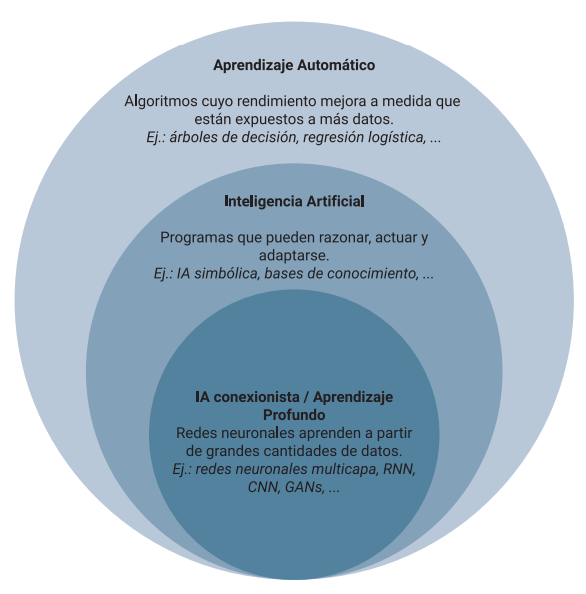
\includegraphics[width=9cm]{figs/Algoritmos de ML.png}
    \end{center}
    \caption{Diagrama de Venn de la relación entre distintas áreas de la IA}
    \label{fig:AlgoritmosML}
\end{figure}
\pagebreak

El Machine Learning, abarca desde enfoques más superficiales hasta técnicas más avanzadas, tal y como se ha podido observar, sin embargo, es el Deep Learning lo que realmente potencia la capacidad de las máquinas para aprender y generalizar patrones complejos de manera excepcional. En la próxima sección, se hablará sobre el Deep Learning, centrándose en las RNA y en cómo estas posibilitan abordar tareas más complejas, como el reconocimiento de patrones en imágenes o el procesamiento de lenguaje natural.

\section{Deep Learning}
\label{sec:DeepLearning} 
El Deep Learning o aprendizaje profundo, constituye una rama de la IA, incluida dentro del Machine Learning, cuyos modelos computacionales se inspiran en el funcionamiento del cerebro humano y se diseñan con el propósito de adquirir conocimientos y llevar a cabo tareas específicas mediante el procesamiento de datos. La etiqueta \textit{profundo} hace referencia a la presencia de múltiples capas de neuronas artificiales en la red, lo que facilita la representación jerárquica de características y potencia la capacidad para aprender y poder diferenciar patrones complejos a partir de los datos.\\

Las Redes Neuronales Artificiales (RNA) o Artificial Neural Networks (ANN) en inglés, están inspiradas en las redes neuronales biológicas del cerebro humano tal y como muestra la Figura \ref{fig:Modelo neurona}, presentando características del mismo, ya que estas aprenden de la experiencia, generalizan de ejemplos previos a ejemplos nuevos y abstraen las características principales de una serie de datos. En las RNA, la unidad análoga a la neurona biológica es el elemento procesador, PE (Process Element). Un PE tiene varias entradas y las combina, normalmente, con una suma básica. La suma de las entradas es modificada por una función de transferencia y el valor de la salida de esta función de transferencia se pasa directamente a la salida del elemento procesador. Existen dos capas con conexiones con el mundo exterior, una capa de entrada o buffer de entrada, donde se presentan los datos a la red, y una capa o buffer de salida que mantiene la respuesta de la red a una entrada, mientras que el resto de las capas reciben el nombre de capas ocultas \cite{Basogain08}.\\

\begin{figure} [H]
    \begin{center}
      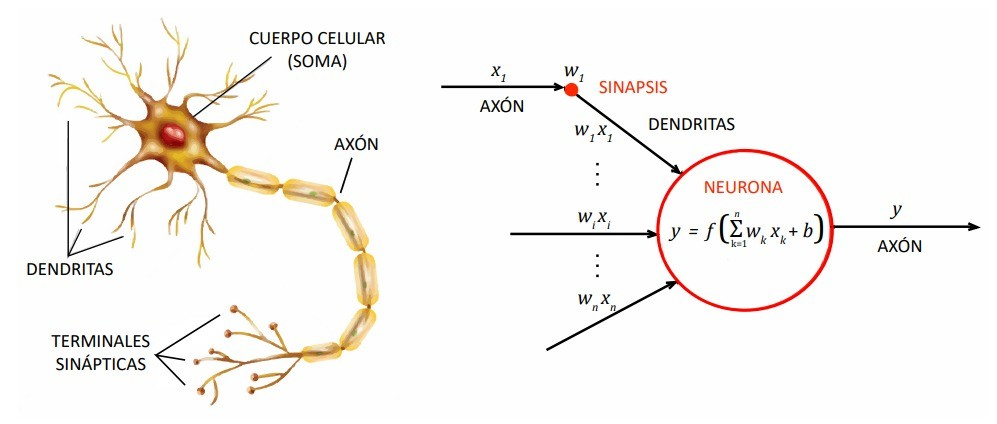
\includegraphics[width=12cm]{figs/Modelo neurona.jpeg}
    \end{center}
    \caption{Modelo biológico de una neurona genérica, comúnmente una neurona motora típica (izquierda) y el respectivo modelo matemático (derecha)}
    \label{fig:Modelo neurona}
\end{figure}

En consecuencia, se puede construir una red neuronal artificial mediante un conjunto de neuronas artificiales, es decir, mediante un conjunto de funciones, y conectando comúnmente la salida de cada una a las entradas de otras diferentes. De esta manera, las RNA no son más que redes de funciones, típicamente representadas mediante la composición de varias funciones como se representa en la Figura \ref{fig:Arquitectura red neuronal}. Esto hace que los diferentes modelos de redes neuronales difieran principalmente en las funciones de activación utilizadas, el patrón de interconexión, e inclusive el tiempo de trasmisión de la información. Es importante señalar que la característica clave de la sinapsis, el escalar las señales de entrada por factores (pesos), es la manera en la que se cree que el cerebro aprende. Por lo tanto, distintos pesos dan como resultado diferentes respuestas a una entrada. De esta manera, se puede decir que el aprendizaje es el ajuste de los pesos en respuesta a un estímulo \cite{Dinamarca18}.\\

\begin{figure} [h!]
    \begin{center}
      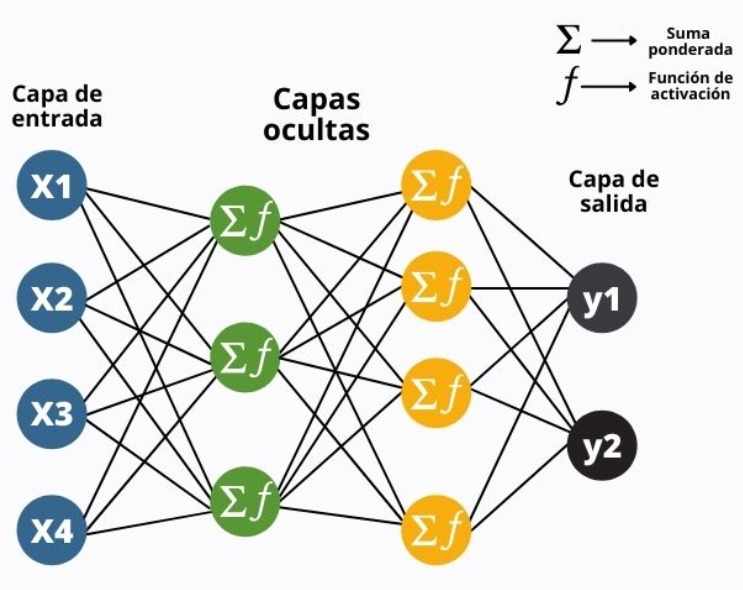
\includegraphics[width=8cm]{figs/capas rrnn.jpeg}
    \end{center}
    \caption{Arquitectura de una red neuronal}
    \label{fig:Arquitectura red neuronal}
\end{figure}

La historia de las redes neuronales se remonta a la década de 1940, cuando el neurofisiólogo Warren McCulloch y el matemático Walter Pitts modelaron una red neuronal simple utilizando circuitos eléctricos. Su modelo estaba basado en la idea de lógica de umbral, que más tarde sería fundamental para el desarrollo de las redes neuronales artificiales. En 1958, el neurobiólogo Frank Rosenblatt dio un paso significativo al comenzar a trabajar en el perceptrón, un modelo computacional que representaba la unidad básica de una red neuronal y realizaba una suma ponderada de varias entradas, al tratarse de una unidad de procesamiento, llevando a cabo una combinación lineal de esas entradas, y aplicando posteriormente una función de activación para producir una salida. Este trabajo marcó el inicio de la investigación en redes neuronales artificiales. Saltando a la década de 2010, dos factores contribuirían a la revolución de aplicaciones de redes neuronales y algoritmos de aprendizaje profundo. En primer lugar, los avances en hardware especializado aceleraron drásticamente el entrenamiento y el rendimiento de las redes neuronales, reduciendo su consumo de energía, mientras que, en segundo lugar, el aumento de datos abiertos disponibles en línea y servicios de bajo costo para etiquetar datos impulsaron el desarrollo de la inteligencia artificial \cite{Abeliuk21}.\\\\
\\

En este capítulo se ha introducido el nacimiento y la historia de los robots y la robótica tal y como los conocemos hoy en día, dentro de cuya rama encontramos uno de los tres grandes grupos en los cuales puede dividirse esta, la Robótica de Servicio, y para la que la Inteligencia Artificial, y más concretamente el campo de la Visión Artificial junto con el del Deep Learning, siendo este subcategoría del Machine Learning, juegan un papel fundamental en el desarrollo de nuevas aplicaciones.\\

En este proyecto se presenta un sistema que, mediante Visión Artificial y Machine Learning, es capaz de reconocer la maduración de frutos, más concretamente de fresas, con el objetivo de poder ayudar así a mejorar el proceso de recolección. En los siguientes capítulos de este trabajo se detallarán los objetivos del mismo, delineando claramente las metas; se expondrá la plataforma de desarrollo, detallando las herramientas seleccionadas para la elaboración del proyecto; se presentará el diseño y la arquitectura del proyecto; y, finalmente, llegaremos a las conclusiones, donde tendrá lugar una breve recopilación de información sobre los resultados obtenidos y las posibles direcciones futuras. 
